\documentclass{beamer}
\usetheme{Madrid}

\usepackage{graphicx}
\usepackage{amsmath}

\title{Matrix Embedding with LSBM and Hamming Codes}
\author{Marcel Auer}
\date{\today}

\begin{document}

\begin{frame}
    \titlepage
\end{frame}

\begin{frame}{1. True Embedding with LSBM and Hamming Codes}
    \textbf{Approach}
    \begin{itemize}
        \item Implemented matrix embedding explicitly by generating parity-check matrices $H$ for Hamming codes.
        \item \textbf{Syndrome Calculation}: Compute $s = H \cdot y \pmod{2}$. The required change is $m - s \pmod{2}$.
        \item \textbf{Modification}: Find the index to change based on the difference. 
        \item \textbf{LSBM}: In LSB Matching, changing the LSB equates to randomly adding or subtracting $1$ from the pixel intensity, ensuring boundaries (like $0$ and $x_{max}$) are respected.
    \end{itemize}
\end{frame}

\begin{frame}{2. Simulating Hamming Codes}
    \textbf{Simulation Strategy}
    \begin{itemize}
        \item Each Hamming code block changes with probability $P(\text{change}) = \frac{2^k - 1}{2^k}$.
        \item The total number of modified blocks can be sampled directly using a Binomial distribution: \\ $\sim \text{Binomial}\left(N_{\text{blocks}}, \frac{2^k - 1}{2^k}\right)$.
        \item Solves the need to explicitly execute code matrices over covers, massively increasing simulation speed.
    \end{itemize}
    \vspace{0.5em}
    \textbf{Interpolation for Target $\alpha$}
    \begin{itemize}
        \item To achieve non-integer embedding rates $\alpha$, we linearly interpolate the change probabilities per element of the two neighboring Hamming codes $k$ and $k+1$.
    \end{itemize}
\end{frame}

\begin{frame}{Embedding efficiency $\varepsilon$ for different $k$}
    \centering
    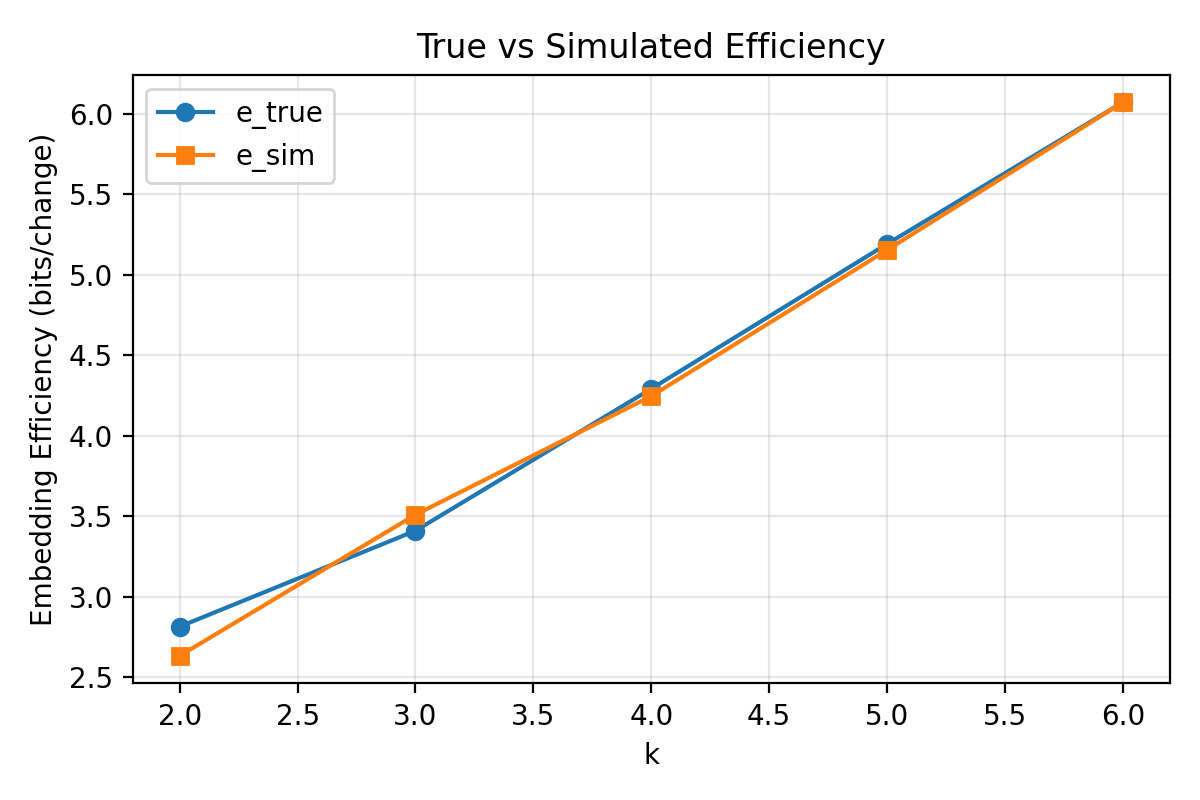
\includegraphics[height=0.36\textheight]{plots/hamming_benchmark_k_efficiency.png}
\end{frame}

\begin{frame} {Speedup of Hamming code simulation}
    \centering
    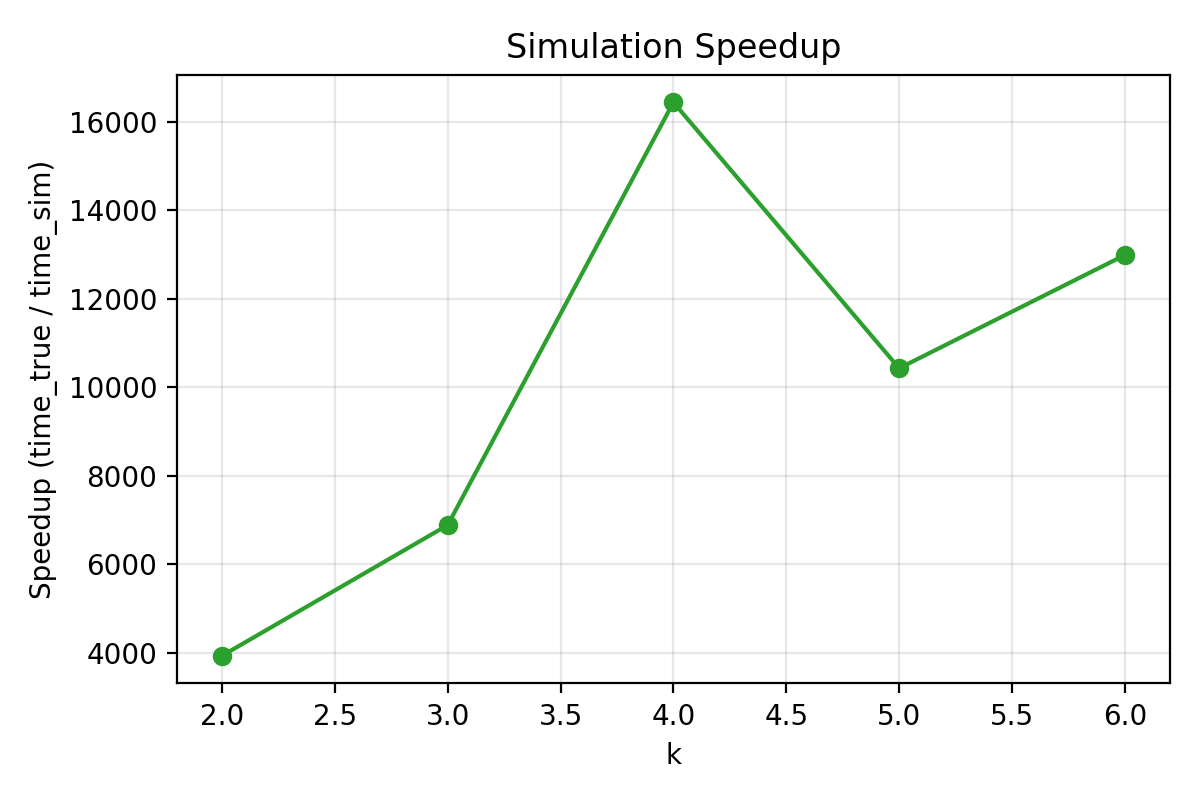
\includegraphics[height=0.36\textheight]{plots/hamming_benchmark_k_speedup.png}
\end{frame}

\begin{frame} {LSBM hamming against reg. LSBM}
    \centering
    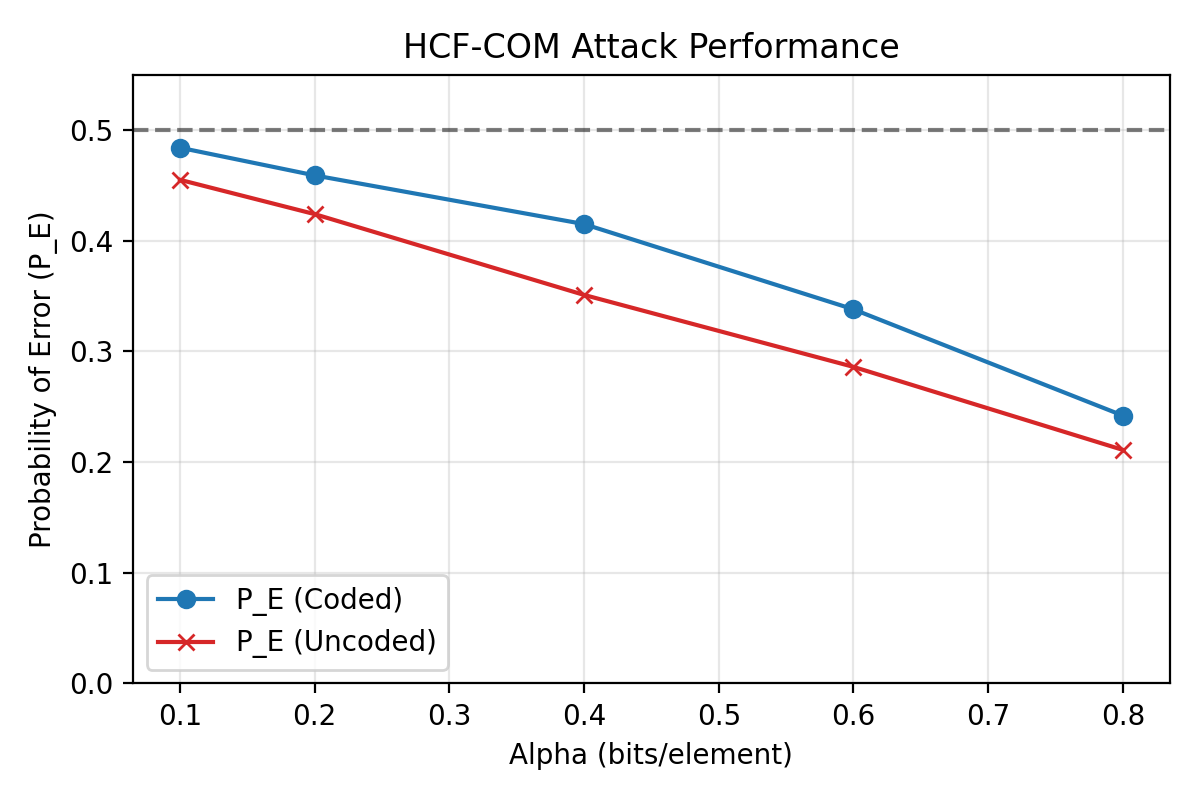
\includegraphics[height=0.36\textheight]{plots/hamming_benchmark_hcf_pe.png}
\end{frame}

\begin{frame}{Conclusion}
    \textbf{Summary}
    \begin{itemize}
        \item \textbf{Completed Implementation:} Fully functional LSB Matching based upon matrix embedding with Hamming codes.
        \item \textbf{Fast Simulator derived:} Allows generating theoretical impacts for arbitrary embedding rates $\alpha$ via local interpolation.
        \item \textbf{Results:} We empirically validated the efficiency of Hamming codes, proving they are substantially safer from detectability and evaluating precisely correctly compared to direct code simulations.
    \end{itemize}
\end{frame}

\end{document}